\documentclass[10pt]{beamer}

% --- Theme and Color Settings ---
\usetheme{Madrid}
\usecolortheme{whale}
\setbeamertemplate{navigation symbols}{} % Remove navigation icons
\setbeamertemplate{caption}[numbered]   % Number figures and tables

% --- Packages ---
\usepackage[utf8]{inputenc}
\usepackage[T1]{fontenc}
\usepackage{booktabs}    % For professional tables
\usepackage{graphicx}    % For images
\usepackage{subcaption}  % For subfigures

% --- Metadata ---
\title[Herbal Plant Recognition]{Comparative Evaluation of ORB-Based BoVW, CNN, and Transfer Learning for Herbal Plant Recognition}
\subtitle{CV Semester Project - Final Exam}
\author[Anonymous]{Henry Ssenono 2025/HD05/26373/U \\ \small{Paper ID *****}}
\date[CVPR 2026]{Jun 7, 2026}

\begin{document}

% Slide 1: Title Slide
\begin{frame}
    \titlepage
\end{frame}

% Slide 2: Abstract Overview
\begin{frame}{Abstract}
    \begin{itemize}
        \item \textbf{Objective:} Automated recognition of herbal plants in diverse environmental conditions.
        \item \textbf{Dataset:} 425 images (14 classes) extracted from 21 video sequences.
        \item \textbf{Methods Investigated:}
            \begin{enumerate}
                \item Traditional ML: ORB features + Bag-of-Visual-Words (BoVW).
                \item Deep Learning: Custom CNN trained from scratch.
                \item Transfer Learning: MobileNetV2 pre-trained on ImageNet.
            \end{enumerate}
        \item \textbf{Key Finding:} Transfer Learning achieved \textbf{93.23\%} test accuracy, vastly outperforming handcrafted and shallow CNN methods.
    \end{itemize}
\end{frame}

% Slide 3: Introduction & Challenges
\begin{frame}{Introduction}
    \begin{block}{The Problem}
        Accurate herbal plant identification is vital for biodiversity, agriculture, and medicine, but remains difficult due to:
    \end{block}
    \begin{itemize}
        \item Lighting variations and viewing angles.
        \item Complex backgrounds and scale changes.
        \item Intra-class variations (plants of same species looking different).
    \end{itemize}
    \begin{block}{Our Contribution}
        A robust preprocessing pipeline and comparative study proving that pre-trained deep representations are superior for small botanical datasets.
    \end{block}
\end{frame}

% Slide 4: Methodology: Dataset Construction
\begin{frame}{Methodology: Dataset}
    \begin{columns}
        \begin{column}{0.5\textwidth}
            \begin{itemize}
                \item \textbf{Source:} 21 video recordings.
                \item \textbf{Classes:} 14 (Pseudo-labeled A--N).
                \item \textbf{Split:} 70\% Train, 15\% Val, 15\% Test.
                \item \textbf{Preprocessing:} HSV-based vegetation filtering and Blur detection (Variance of Laplacian).
            \end{itemize}
        \end{column}
        \begin{column}{0.5\textwidth}
            \begin{figure}
                \centering
                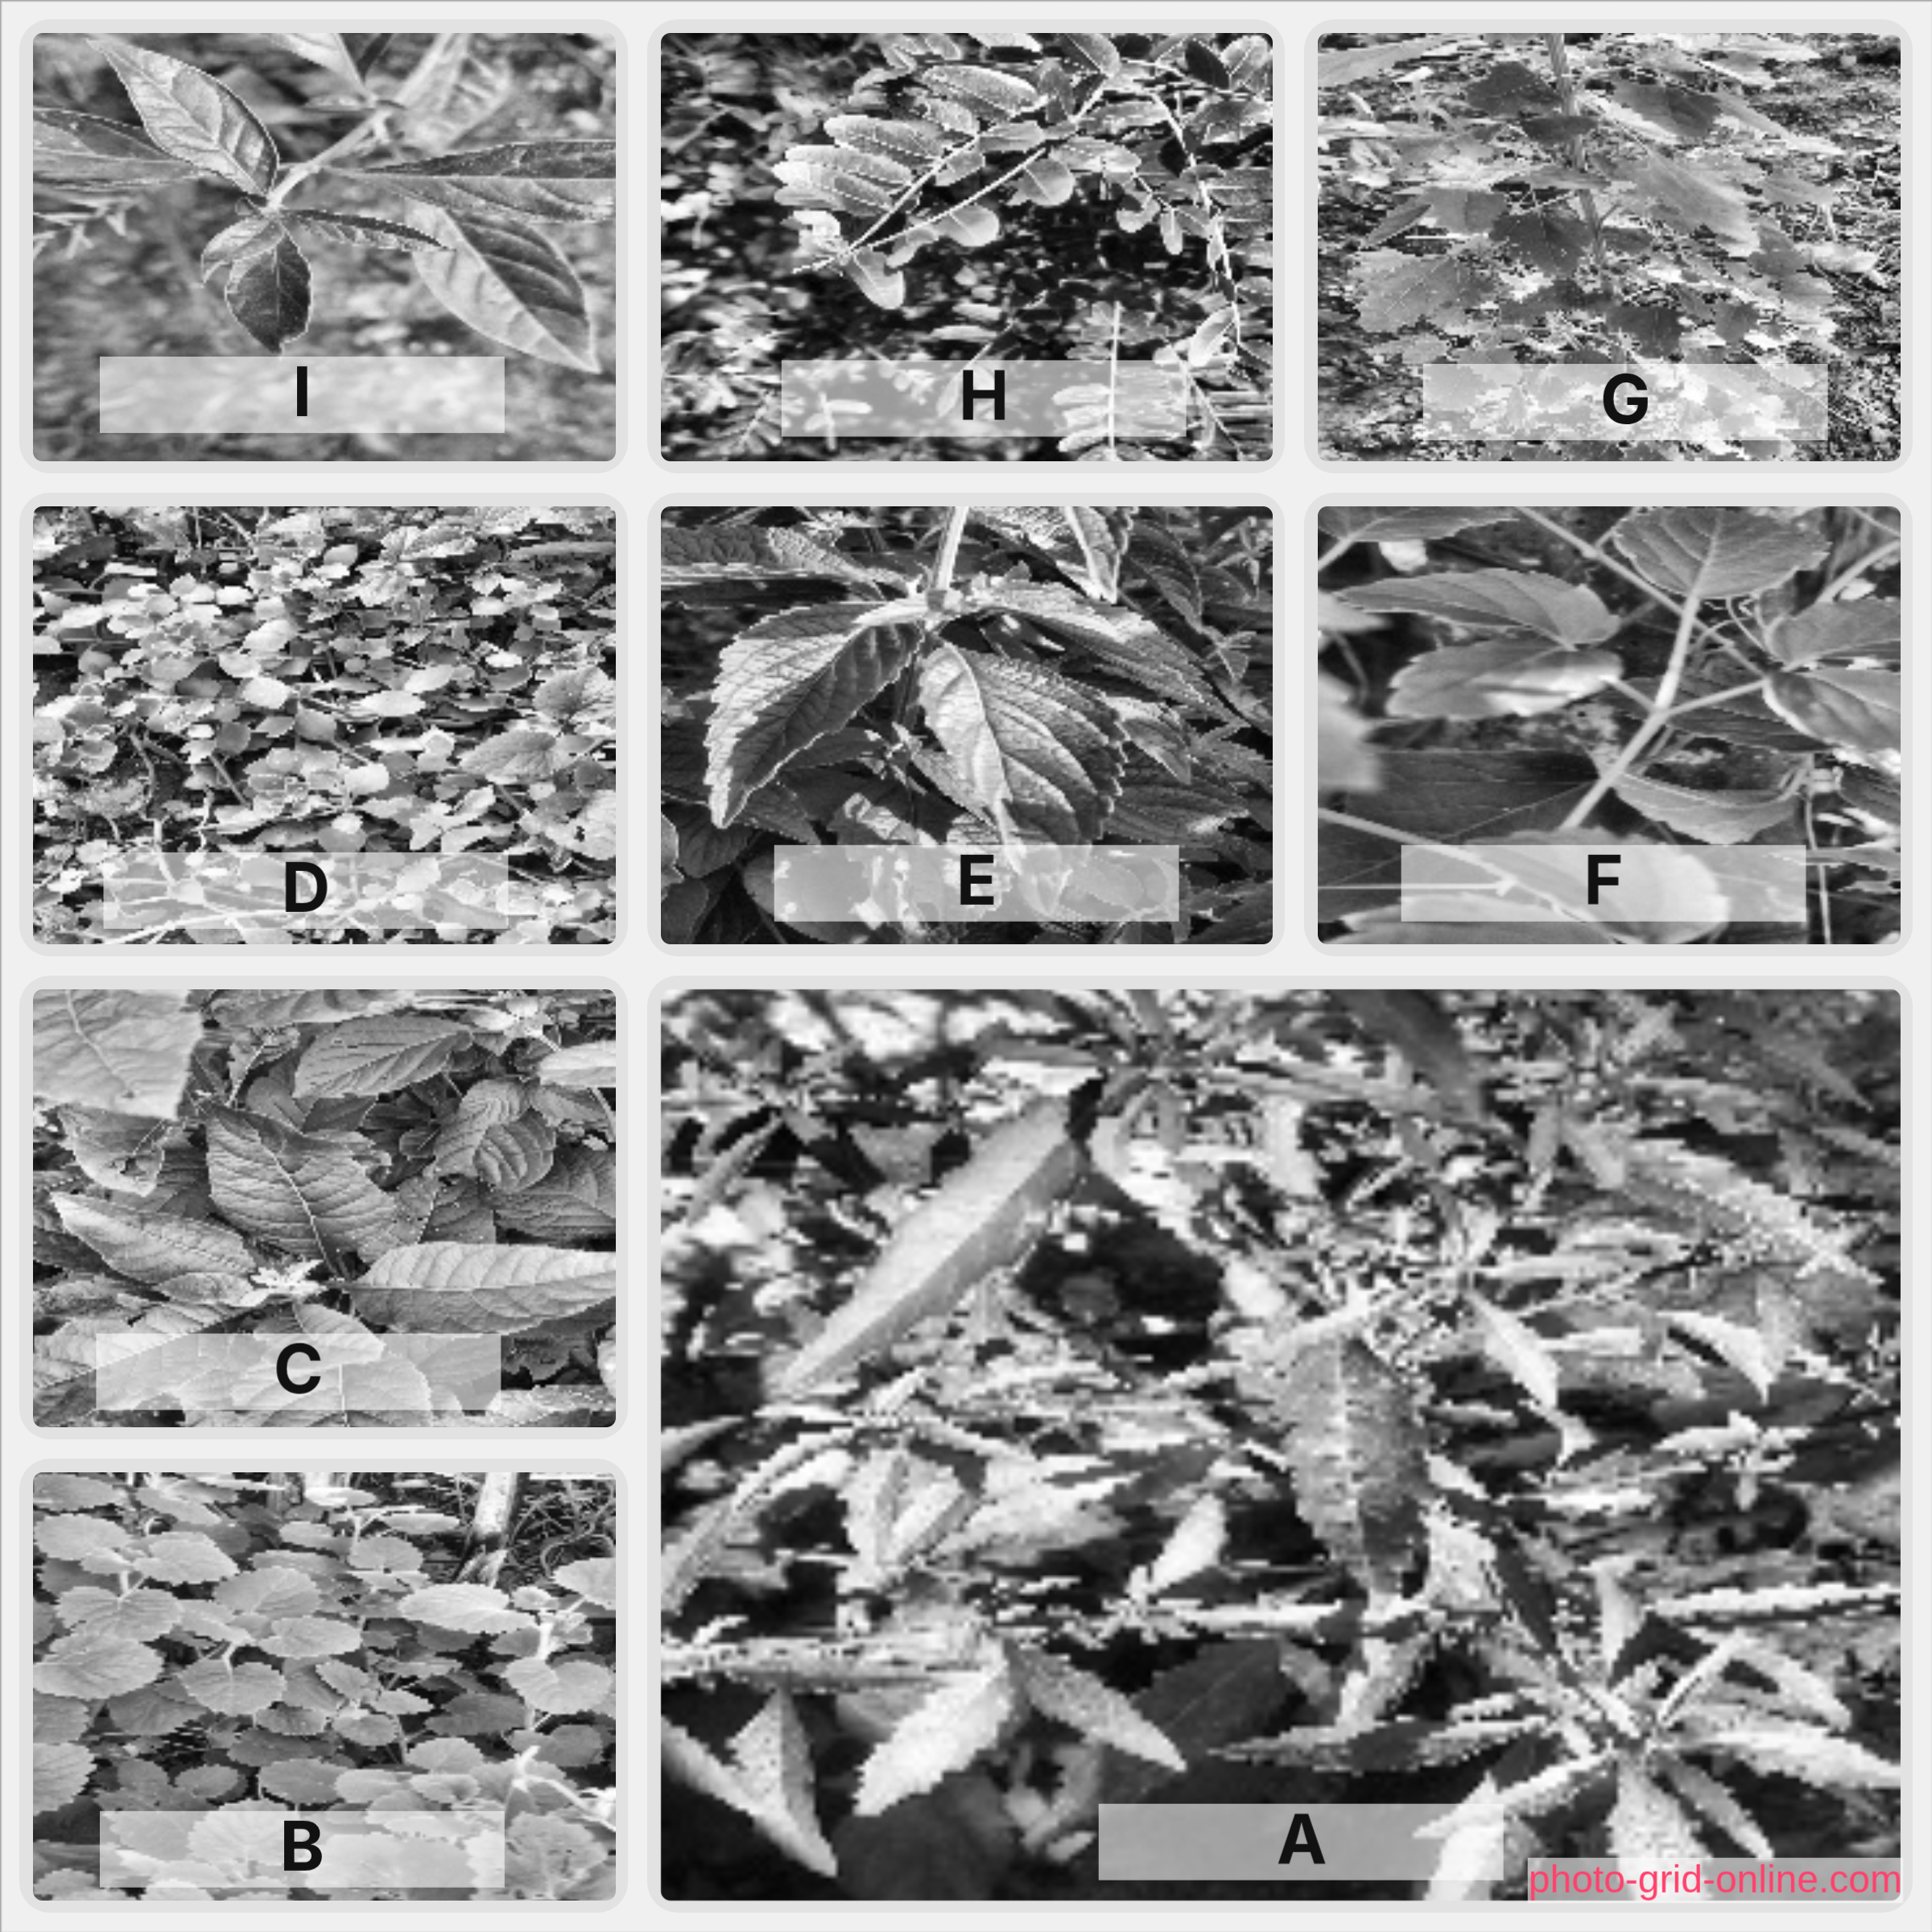
\includegraphics[width=0.8\linewidth]{media/samples.png}
                \caption{Sample herbal plant images from different classes.}
            \end{figure}
        \end{column}
    \end{columns}
\end{frame}

% Slide 5: Dataset Statistics (Table 1)
\begin{frame}{Dataset Statistics}
    \begin{table}
        \centering
        \caption{Image count per pseudo-label class.}
        \small
        \begin{tabular}{lc@{\hspace{2em}}lc}
            \toprule
            \textbf{Class} & \textbf{Count} & \textbf{Class} & \textbf{Count} \\
            \midrule
            A & 11 & H & 30 \\
            B & 43 & I & 9  \\
            C & 27 & J & 16 \\
            D & 37 & K & 38 \\
            E & 33 & L & 40 \\
            F & 34 & M & 47 \\
            G & 29 & N & 31 \\
            \midrule
            \textbf{Total} & & & \textbf{425} \\
            \bottomrule
        \end{tabular}
    \end{table}
\end{frame}

% Slide 6: Preprocessing Pipeline
\begin{frame}{Preprocessing Pipeline}
    \begin{itemize}
        \item \textbf{Vegetation Filtering:} HSV color thresholding (green pixel ratio) to discard frames without plants.
        \item \textbf{Blur Detection:} Used the Laplacian operator to compute image variance; discarded low-frequency frames.
        \item \textbf{Normalization:} Resized to $224 \times 224$; scaled intensities to $[0, 1]$.
        \item \textbf{Data Augmentation:}
            \begin{itemize}
                \item Horizontal flipping and $\pm 20^\circ$ rotation.
                \item Brightness adjustments and Gaussian blur.
            \end{itemize}
    \end{itemize}
\end{frame}

% Slide 7: Approach 1: Traditional BoVW
\begin{frame}{Approach 1: ORB + BoVW Pipeline}
    \begin{enumerate}
        \item \textbf{Feature Extraction:} 1000 ORB keypoints per image (pool of 232,788 descriptors).
        \item \textbf{Visual Vocabulary:} MiniBatch K-Means to create 500 ``Visual Words.''
        \item \textbf{Classification:} Fixed-length histogram vectors fed into classical models.
    \end{enumerate}
    \begin{table}
        \centering
        \caption{Traditional classifier validation results.}
        \begin{tabular}{lc}
            \toprule
            \textbf{Model} & \textbf{Val Accuracy (\%)} \\
            \midrule
            \textbf{SVM} & \textbf{47.92} \\
            Logistic Regression & 45.83 \\
            Random Forest & 31.77 \\
            Gradient Boosting & 28.65 \\
            \bottomrule
        \end{tabular}
    \end{table}
\end{frame}

% Slide 8: Approach 2: Custom CNN Architecture
\begin{frame}{Approach 2: Custom CNN}
    \begin{figure}
        \centering
        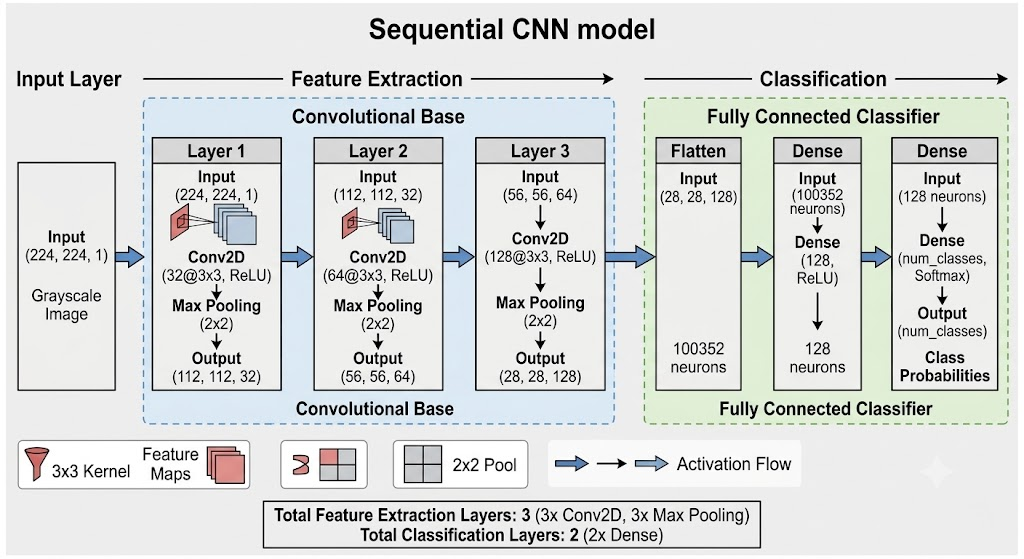
\includegraphics[width=0.9\linewidth]{media/cnn-arch.jpeg}
        \caption{Architecture: 3 Conv Blocks (32, 64, 128) + 2 Dense Layers.}
    \end{figure}
    \begin{itemize}
        \item Trained from scratch using Adam optimizer.
        \item Categorical cross-entropy loss.
        \item Softmax output for 14 classes.
    \end{itemize}
\end{frame}

% Slide 9: Approach 3: MobileNetV2 Transfer Learning
\begin{frame}{Approach 3: MobileNetV2 Transfer Learning}
    \begin{itemize}
        \item \textbf{Base:} MobileNetV2 pre-trained on ImageNet (Frozen).
        \item \textbf{Input:} Grayscale converted to 3-channel RGB.
        \item \textbf{Head:} GlobalAvgPooling $\rightarrow$ Dropout (0.5) $\rightarrow$ Dense (Softmax).
    \end{itemize}
    \begin{figure}
        \centering
        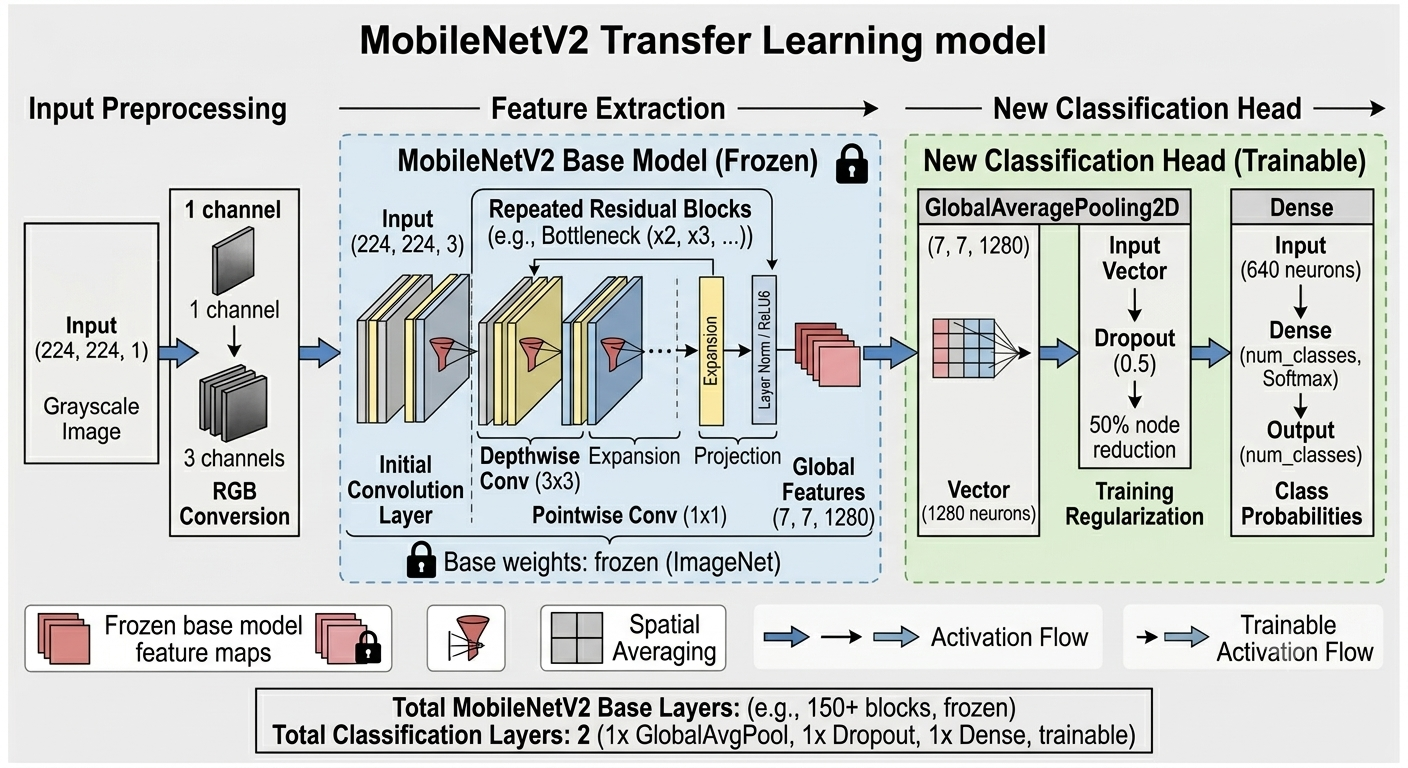
\includegraphics[width=0.8\linewidth]{media/mobilenetv2-transfer-learning.png}
        \caption{MobileNetV2 transfer learning architecture overview.}
    \end{figure}
\end{frame}

% Slide 10: Experimental Results: Comparison
\begin{frame}{Final Model Comparison}
    \begin{table}
        \centering
        \caption{Final comparison on the test set.}
        \begin{tabular}{lc}
            \toprule
            \textbf{Method} & \textbf{Test Accuracy (\%)} \\
            \midrule
            \textbf{MobileNetV2 (Transfer Learning)} & \textbf{93.23} \\
            SVC (BoVW) & 36.46 \\
            Custom CNN (From Scratch) & 22.40 \\
            \bottomrule
        \end{tabular}
    \end{table}
    \begin{block}{Observations}
        \begin{itemize}
            \item Custom CNN suffered from overfitting due to small dataset size (425 images).
            \item Handcrafted ORB features failed to capture fine-grained botanical semantic details.
        \end{itemize}
    \end{block}
\end{frame}

% Slide 11: CNN Training Analysis
\begin{frame}{CNN Learning Curves}
    \begin{figure}
        \centering
        \begin{subfigure}{0.48\textwidth}
            \centering
            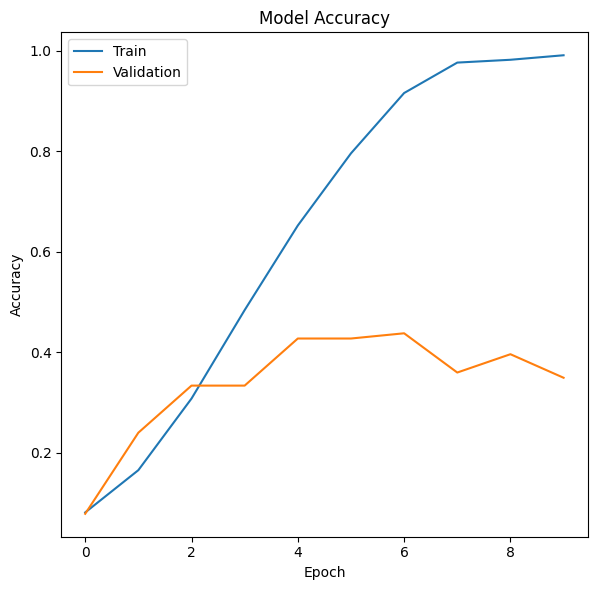
\includegraphics[width=\linewidth]{media/cnn-acc.png}
            \caption{Accuracy (Train/Val)}
        \end{subfigure}
        \hfill
        \begin{subfigure}{0.48\textwidth}
            \centering
            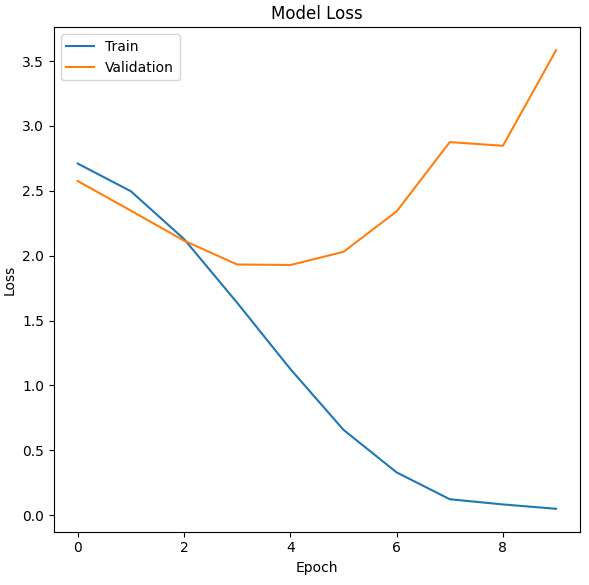
\includegraphics[width=\linewidth]{media/cnn-loss.png}
            \caption{Loss (Train/Val)}
        \end{subfigure}
        \caption{Custom CNN results showing significant overfitting/generalization gap.}
    \end{figure}
\end{frame}

% Slide 12: Conclusion & Future Work
\begin{frame}{Conclusion}
    \begin{itemize}
        \item \textbf{Summary:} Transfer Learning is essential for botanical recognition when dataset size is limited.
        \item \textbf{Performance Gain:} MobileNetV2 improved accuracy by \textbf{+56.77\%} over traditional BoVW.
        \item \textbf{Reproducibility:} The proposed preprocessing pipeline significantly improved image quality for feature learning.
    \end{itemize}
    \begin{block}{Future Directions}
        \begin{itemize}
            \item Expand dataset with more diverse environmental conditions.
            \item Investigate Vision Transformers (ViT) or EfficientNet.
            \item Real-time implementation for mobile plant identification.
        \end{itemize}
    \end{block}
\end{frame}

% Slide 13: Final Slide
\begin{frame}
    \centering
    \Large \textbf{Thank You!}\\
    \vspace{2em}
    \footnotesize CV Semester Project \#*****
\end{frame}

\end{document}